\documentclass{article}

\usepackage{graphicx}
\usepackage{tikz}
\usepackage{tikzsymbols}
\usetikzlibrary{calc,patterns,shapes.geometric}
\pagestyle{empty}
\usepackage[margin=0pt]{geometry}
\geometry{papersize={14in,12in}}

\def\centerarc[#1](#2)(#3:#4:#5){\draw[#1] ($(#2)+({#5*cos(#3)},{#5*sin(#3)})$) arc (#3:#4:#5);}

\begin{document}
	\begin{figure}
		\centering
		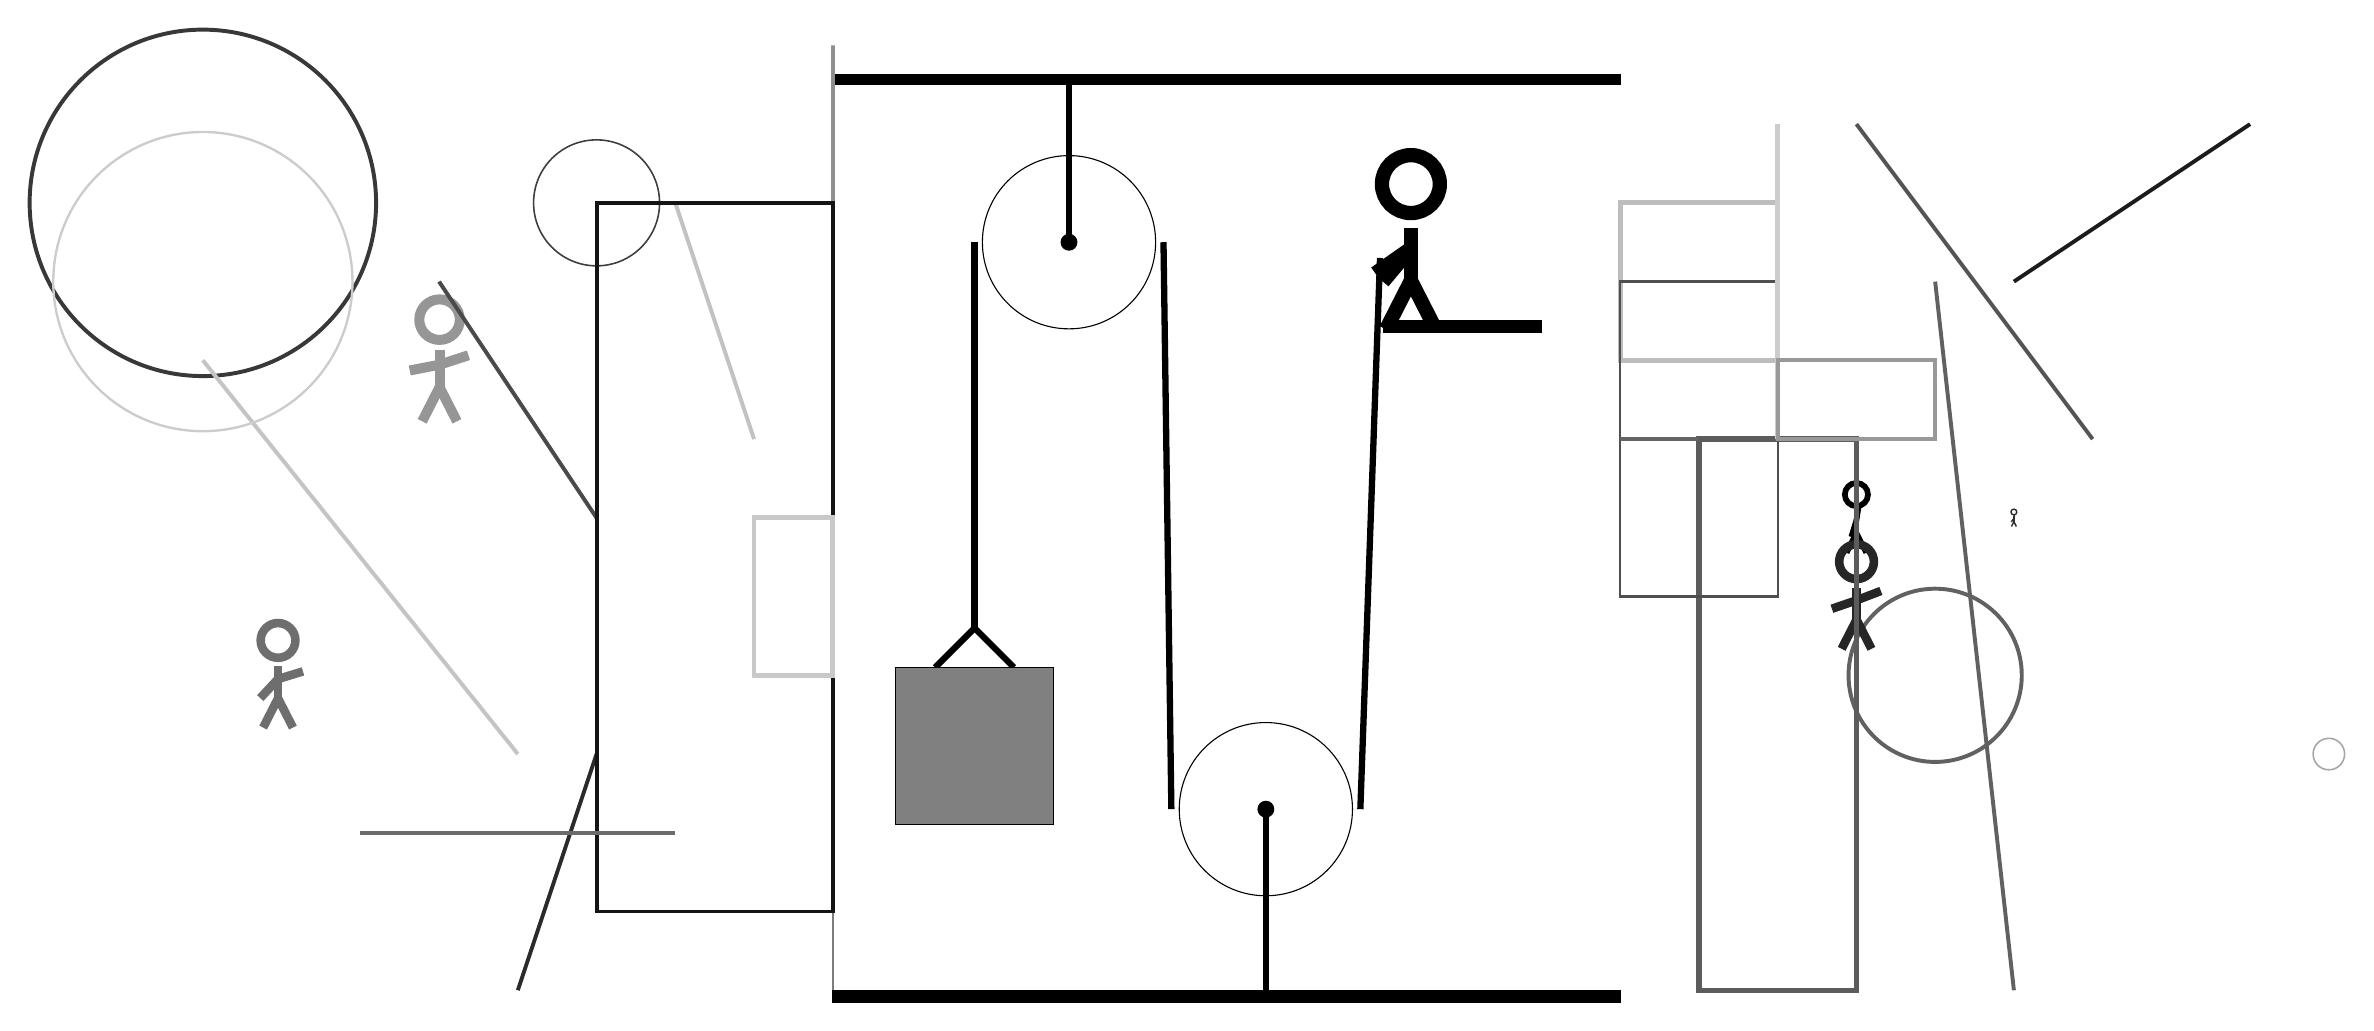
\begin{tikzpicture}
			%%%%% START %%%%%
			
			\draw[fill=black] (-2, 11.5) rectangle (8, 11.625);
			
			\draw (3.5, 2.3) circle (1.1);
			\draw[fill=black] (3.5, 2.3) circle (0.1);
			\draw[line width=0.8mm] (3.5, 2.3) -- (3.5, 0);
			
			\draw (1, 9.5) circle (1.1);
			\draw[fill=black] (1, 9.5) circle (0.1);
			\draw[line width=0.8mm] (1, 11.5) -- (1, 9.5);
			
			\draw[line width=0.8mm](-0.7, 4.1) --  (-0.2, 4.6) -- (0.3, 4.1);
			\draw[fill=black!50] (-1.2, 4.1) rectangle (0.8, 2.1);
			
			\draw[line width=0.5mm, color=black!85](-6, 2) -- (-8, 2);
			
			\draw [line width=0.5mm, color=black!78](-10, 10) circle (2.2);
			\node[line width=0.3mm, color=black!41] at (-7, 8) {\Strichmaxerl[7][11][18]};
			\draw [line width=0.5mm, color=black!62](12, 4) circle (1.1);
			\draw[line width=0.5mm, color=black!44] (-2, 7) rectangle (-2, 12);
			\draw[line width=0.5mm, color=black!83](-5, 3) -- (-6, 0);
			
			\draw [line width=0.2mm, color=black!76](-5, 10) circle (0.8);
			\node[line width=0.6mm, color=black!100] at (11, 6) {\Strichmaxerl[4][73][81]};
			\node[line width=0.6mm, color=black!85] at (11, 5) {\Strichmaxerl[6][19][21]};
			\draw[line width=0.5mm, color=black!71](-5, 6) -- (-7, 9);
			\draw[line width=0.5mm, color=black!24](-3, 7) -- (-4, 10);
			\node[line width=0.4mm, color=black!57] at (-9, 4) {\Strichmaxerl[6][47][17]};
			\node[line width=0.7mm, color=black!82] at (13, 6) {\Strichmaxerl[1][53][80]};
			
			\draw [line width=0.2mm, color=black!35](17, 3) circle (0.2);
			\draw[line width=0.7mm, color=black!64] (9, 0) rectangle (11, 7);
			\draw[line width=0.2mm, color=black!51] (-2, 0) rectangle (-2, 2);
			\draw[line width=0.6mm, color=black!26] (10, 8) rectangle (8, 10);
			\draw[line width=0.3mm, color=black!69] (8, 5) rectangle (10, 9);
			\draw[line width=0.5mm, color=black!92] (-2, 10) rectangle (-5, 1);
			\draw[line width=0.6mm, color=black!20] (10, 11) rectangle (10, 7);
			\draw[line width=0.6mm, color=black!21] (-3, 6) rectangle (-2, 4);
			\draw[line width=0.5mm, color=black!58](-4, 2) -- (-8, 2);
			
			\draw[line width=0.5mm, color=black!61](8, 7) -- (9, 7);
			\draw[line width=0.5mm, color=black!23](-6, 3) -- (-10, 8);
			\draw [line width=0.3mm, color=black!20](-10, 9) circle (1.9);
			\draw[line width=0.5mm, color=black!62](12, 9) -- (13, 0);
			
			\draw[line width=0.5mm, color=black!67](11, 11) -- (14, 7);
			\draw[line width=0.5mm, color=black!89](13, 9) -- (16, 11);
			\draw[line width=0.5mm, color=black!40] (10, 7) rectangle (12, 8);
			
			
			\draw[line width=0.8mm](-0.2, 9.5) -- (-0.2, 4.6);
			\centerarc[line width=0.8mm](1, 9.5)(180:0:1.2000000000000002)
			\draw[line width=0.8mm](2.2, 9.5) -- (2.3, 2.3);
			\centerarc[line width=0.8mm](3.5, 2.3)(180:360:1.2000000000000002)
			\draw[line width=0.8mm](4.7, 2.3) -- (4.95, 9.3);
			
			\node at (5.3, 9.5) {\Strichmaxerl[10][35][-130]};
			\draw[fill=black] (5, 8.5) rectangle (7, 8.35);
			
			\draw[fill=black] (-2, 0) rectangle (8, -0.15);
			
			%%%%% END %%%%%
		\end{tikzpicture}
	\end{figure}	
\end{document}